\documentclass[../rapport_MVEX01-11-05]{subfiles}
\begin{document}

\section{Implementering av HMM för klassificering av icke-statiska gester}

För att klassificera dynamiska gester bygger man vidare på metoden som användes
för de statiska.  HMM kräver att gester utgörs av följder av symboler,
motsvarande olika observationer. Dessa symboler tar vi från en första
klassificering med \knn.

Idén är att representera varje gest, statisk som dynamisk, i form av en
symbolföljd.  De statiska definieras lättast som två eller tre efterföljande
symboler av samma typ, medan de dynamiska består av en följd av blandade
symboler.

Då de statiska gesterna redan tilldelats
symboler ligger problemet i att tilldela icke-statiska gester symboler på ett effektivt sätt. Vår tanke
var att dela upp filmerna med en icke-statisk gest i tre kategorier; prototypfilmer, träningsfilmer och 
testfilmer. Tilldelningen sker genom att varje prototypfilm delas upp i fyra lika stora delar. Den 
första fjärdedelen tilldelas en symbol, den andra en annan osv. Förhoppningen är att liknande 
delgester (behöver omformuleras) på så vis tilldelas samma symbol. 

Programmet omvandlar därefter träningsfilmerna till symboler via kodboken som utvidgats 
med prototypgesterna. Längden av 
symbolföljden för respektive gest beror på programmets prestanda, dvs hur många bilder 
man önskar analysera per sekund. Det bör uppmärksammas att varianter av en och samma gest 
kommer, beroende på deras längd, representeras av olika långa symbolföljder, vilket leder till 
att vi tränar flera HMM-modeller för varje gest. En möjlighet är att gruppera in symbolsekvenserna 
i tre längder för att motverka alltför strikta krav på gestens utförande. 

HMM-modellerna tränas med Baum-Welch-metoden via \MATLAB-funktionen \texttt{hmmtrain}. Vi använder Bakis-modellen 
då den som sagt gett bra resultat i samband med signaler som förändras över tid, en topologi som medför att
modellerna måste tränas med flera symbolsekvenser \cite{Rabiner89}. Då ingen förflyttning till ett tidigare
tillstånd är tillåten blir modellen nämligen mycket selektiv med vilka symboler varje tillstånd kan generera. 
Enbart en symbolföljd skulle träna modellen till att systematiskt vandra från ett tillstånd till nästa och i 
varje generera rätt symbol i ordningen med sannolikhet ett. 

\notes{Nämna att vi skrev egen HMM-kod}

För att beräkna sannolikheten att en viss HMM skapat en symbolföljd används \MATLAB-funktionen \texttt{hmmviterbi}. 
Om vi antar att det tränats HMMs för gester av längd två, fem och sju symboler kommer programmets klassificering 
av testfilmerna ske på det sätt som beskrivs i
figur~\vref{fig:hmm-flowchart}.
 
 \begin{figure}[tbp]
  \centering
  \captionsetup{singlelinecheck=off} % hack
  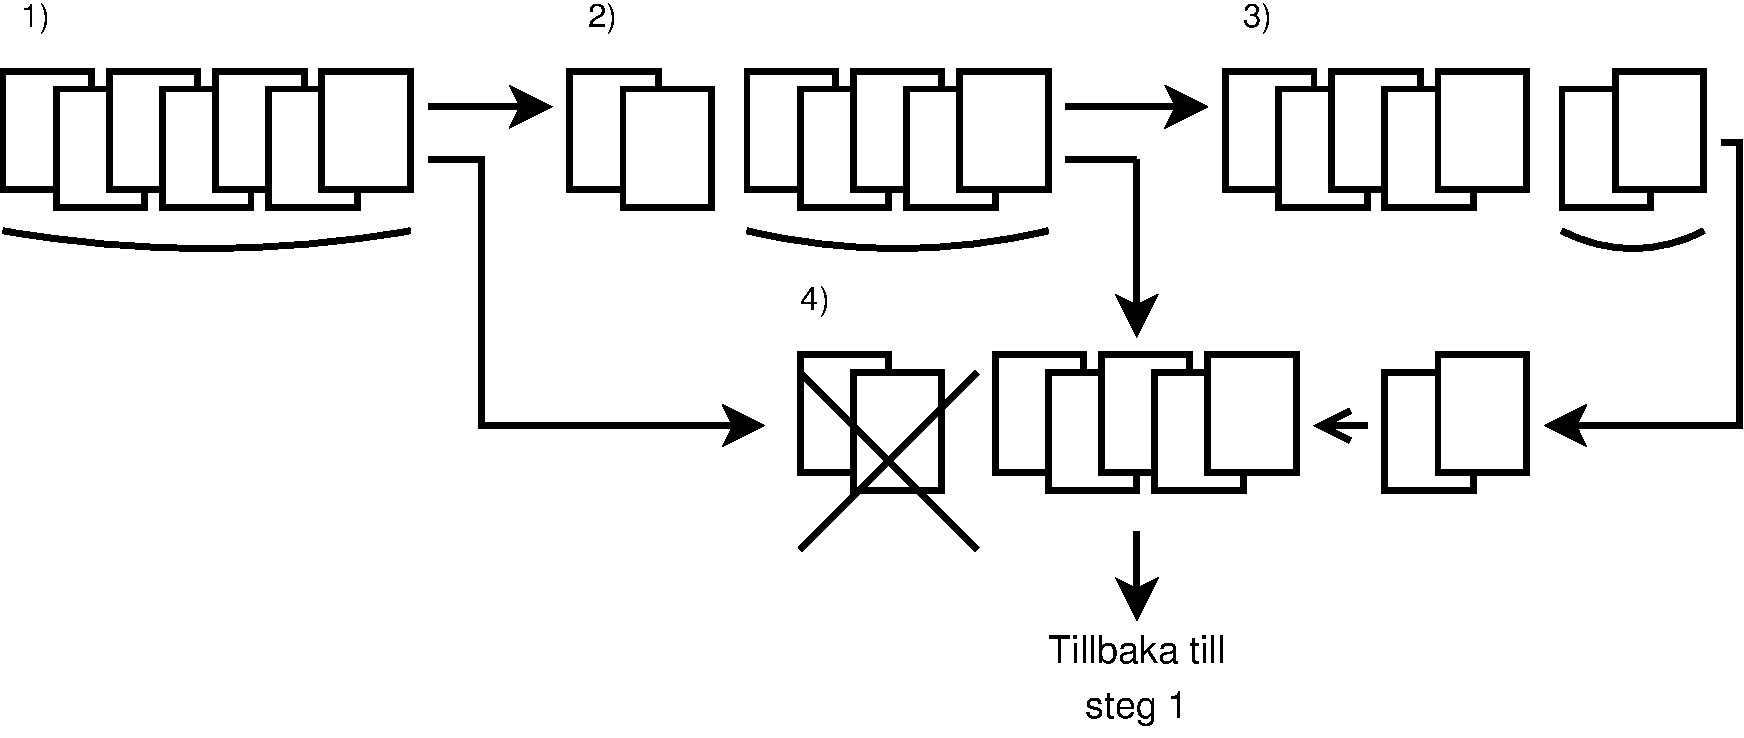
\includegraphics[width=0.95\textwidth]{bilder/HMM_flowchart}
  \caption[Klassificering av dynamiska gester med två, fem och sju
  symboler]{Klassificering av dynamiska gester med två, fem och sju
  symboler sker enligt en relativt enkel procedur:
  \begin{enumerate}
    \item Programmet beräknar sannolikheten att en HMM tränad med sju
	symboler skapat symbolföljden. Är någon sannolikhet tillräckligt hög 
	registreras den aktuella gesten och programmet går till steg fyra, 
	annars går det vidare till steg två.
    \item Programmet beräknar sannolikheten att de fem senaste symbolerna
	skapats av en HMM tränad med fem symboler. Vid tillräckligt hög sannolikhet 
	registreras en gest och programmet går till steg fyra, annars går det 
	vidare till steg tre. 
    \item Programmet beräknar sannolikheten att de två senaste symbolerna skapats av 
	en HMM tränad med två symboler. Om sannolikheten är tillräckligt hög registreras
	en (statisk) gest. 
    \item De två äldsta symbolerna kasseras och två nya sätts in i slutet av följden. 
	Programmet börjar om från steg ett.
  \end{enumerate}
	 Märk att denna algoritm prioriterar långa symbolföljder,
	dvs.~störst går först.}
  \label{fig:hmm-flowchart}
\end{figure}
 
 \end{document}

